\chapter{Equação da Onda em Meios Não-Homogêneos}

    \label{cap:CompMDFeRT}

    \section{Resolução da Equação da Onda por Diferenças Finitas}
    
        Como já dito, o objetivo desse trabalho é a comparação de métodos que consigam resolver a equação da onda com fonte, 
        simulando a propagação de oscilações através de meios acamadados de composição não-homogênea. Portanto, 
        seguindo o escopo desse objetivo, apresentaremos nesse relatório apenas as simulações para o caso em duas 
        dimensões das oscilações, como se dá no estudo da sísmica.
    
        \subsection{Reflexão na Borda do Domínio de Propagação da Onda}
	        
            Suponhamos um meio acamadado cujas interfaces, na forma de retas que podem ser representadas por funções, 
            se distribuem como na figura abaixo:
            \begin{figure}[H]
                \centering
                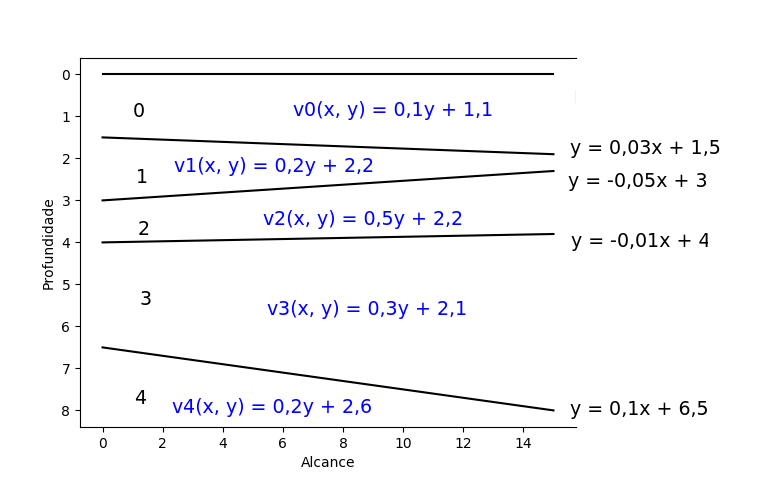
\includegraphics[scale=.7]{imagens/ilustracoes/TR.png}
                \caption{Meio acamadado com interfaces retas (em preto) representadas por funções e camadas representadas
                por números de 0 a 4. As funções de velocidade de cada camada também são apresentadas na imagem}
                \label{fig:interfacesAndMedium}
            \end{figure}
            Além da distribuição das interfaces, a imagem também apresenta como se dá a propriedade de não-homogeneidade do 
            meio através das funções de velocidades para cada camada. Em um ambiente real, a não-homogeneidade se dá através 
            da formação das camadas por diversos tipos de materiais que estão misturados e cuja distribuição depende da posição 
            em que se encontram e da pressão que sofrem.
            
            As bordas do meio definido refletem as ondas. Para tal, podemos pensar o meio por onde a onda propagará como uma
            cama elástica, que é presa em suas bordas. Para imitar isso, usamos as condições de contorno como em (\ref{eq:condContorno})
            que pode ser implementado em código: imagine um \textit{array} tridimensional (visto que o problema se dá em $x$, $y$ e $t$)
            no qual, para cada posição no eixo que representa $t$ exista um \textit{array} $xy$ que representa o nosso meio. Então aplicamos as
            condições de contorno zerando as ``bordas'' de cada um desses arrays.
            
            Para que simulemos o espalhamento das oscilações precisamos de uma fonte as inicie. Para isso, podemos utilizar a \textit{wavelet} 
            de Ricker (também conhecida como \textit{mexican hat wavelet}) como fonte. Essa \textit{wavelet} é dada pela função
            \begin{equation}
                \label{eq:rickerWavelet}
                f(t) = (1 - 2\pi^2f_M^2t^2)^{-\pi^2f_M^2t^2}
            \end{equation}
            na qual, $t$ representa o tempo e $f_M$ representa a frequência de pico \cite{rickerWLet}. Podemos visualisar um exemplo da \textit{wavelet} na Figura \ref{fig:Ricker}
            \begin{figure}[H]
                \centering
                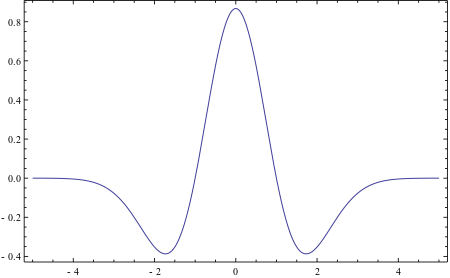
\includegraphics[scale=.6]{imagens/MexicanHatMathematica.png}
                \caption{Exemplo da \textit{wavelet} de Ricker, por JonMcLoone [CC BY-SA 3.0 (https://creativecommons.org/licenses/by-sa/3.0)], via Wikimedia Commons}
                \label{fig:Ricker}
            \end{figure}
            
            Suponhamos também que esse meio está englobado por um sistema de coordenadas cartesianas cuja origem se encontra
            no extremo esquerdo superior da imagem (\ref{fig:interfacesAndMedium}) e cujo eixo das ordenadas aponta para baixo. 
            Assume-se o eixo assim porque a simulação da propagação de ondas se dará por todo o meio, que é subterrâneo, e para 
            baixo.
	        
            \subsubsection{Prática Numérica}
            
                Utilizando o arquivo \textit{userInput.py}, recebemos os parâmetros para a onda e o meio que o usuário deseja que a simulação siga, gerando um arquivo \textit{data.npy}. Após isso executamos o arquivo \textit{reflect.py}, que lerá o arquivo \textit{data.py}, criará o meio e a onda como desejado e realizará a simulação usando o método de diferenças finitas. Por fim o programa salva um arquivo \textit{U.npy}, que contém a simulação da propagação de ondas. Esse último arquivo pode ser usado pelo programa \textit{snapshoter.py} para gerar \textit{snapshots} (``fotografias'') das superfícies de contorno da onda.
                
                Os \textit{snapshots} da Figura \ref{fig:snapsMDF} foram criados para uma simulação da propagação, com no máximo 90 s, de uma onda com frequência dominante de um hertz, amplitude de um quilômetro, pico da fonte na origem do meio que tem 15 km de extensão e 9,5 km de profundidade. As velocidades do meio se distribuem de acordo com o que podemos ver na imagem \ref{fig:velDist}.
                
                \begin{figure}[H]
                    \centering    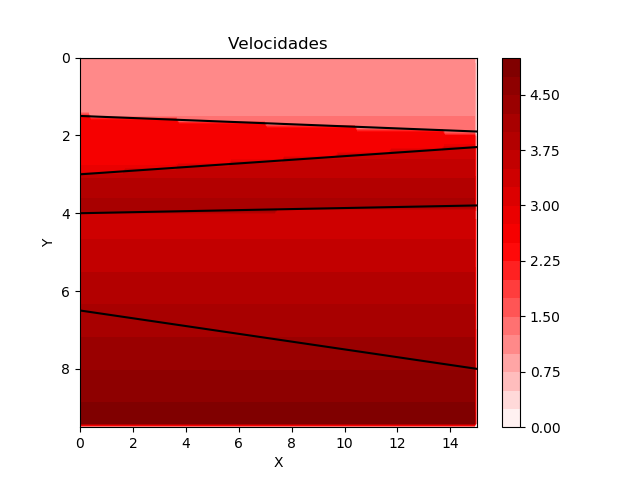
\includegraphics[scale=.8]{imagens/FDMimages/Velocidades.png}
                    \caption{Distribuição das velocidades no meio usado como exemplo}
                    \label{fig:velDist}
                \end{figure}
                
                \begin{figure}[H]
                    \begin{tabular}{cc} 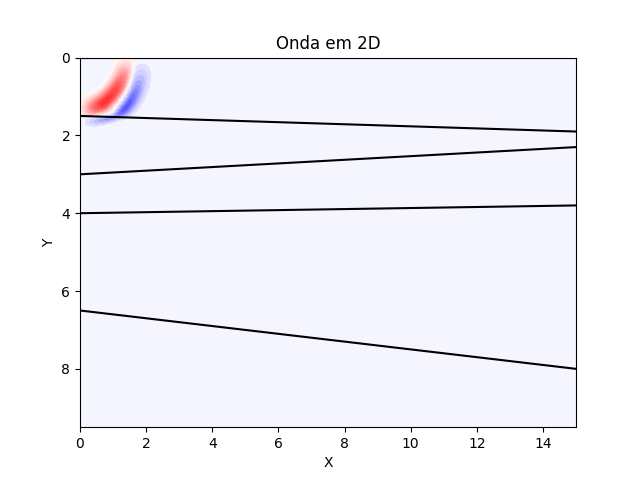
\includegraphics[width=65mm]{imagens/FDMimages/Teste00.png} &  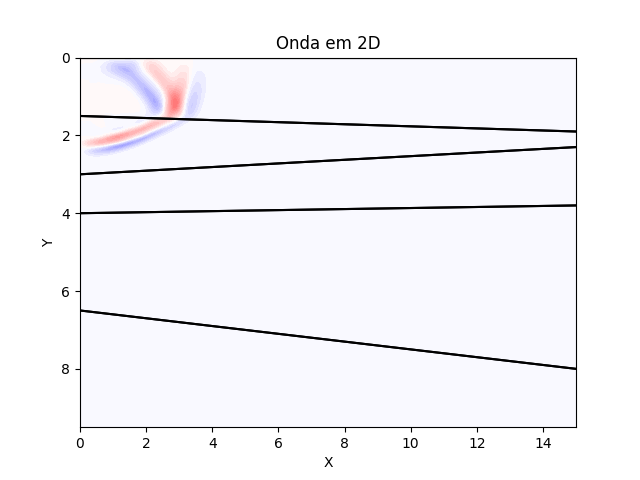
\includegraphics[width=65mm]{imagens/FDMimages/Teste01.png} \\
                    (a) 1 & (b) 2 \\
                    [6pt] 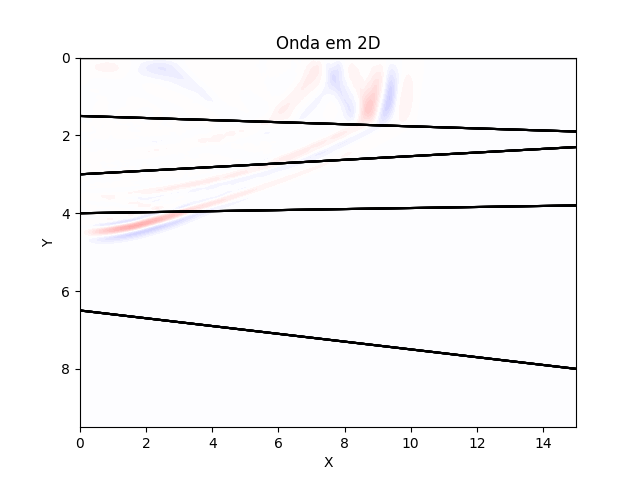
\includegraphics[width=65mm]{imagens/FDMimages/Teste05.png} & 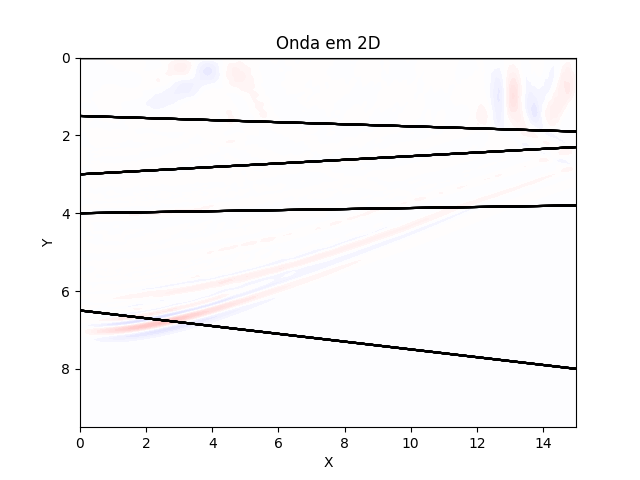
\includegraphics[width=65mm]{imagens/FDMimages/Teste010.png} \\
                    (c) 3 & (d) 4 \\
                    [6pt] 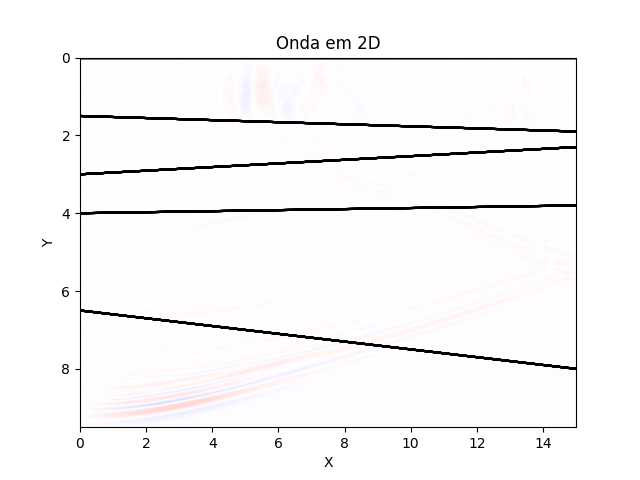
\includegraphics[width=65mm]{imagens/FDMimages/Teste015.png} & 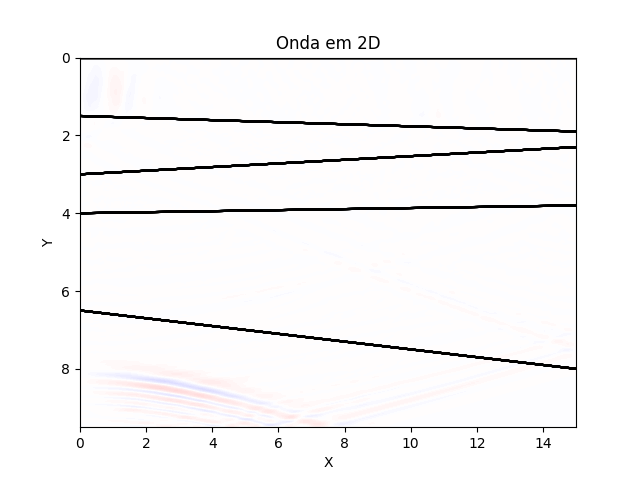
\includegraphics[width=65mm]{imagens/FDMimages/Teste019.png} \\ 
                    (e) 5 & (f) 6\\
                    [6pt] 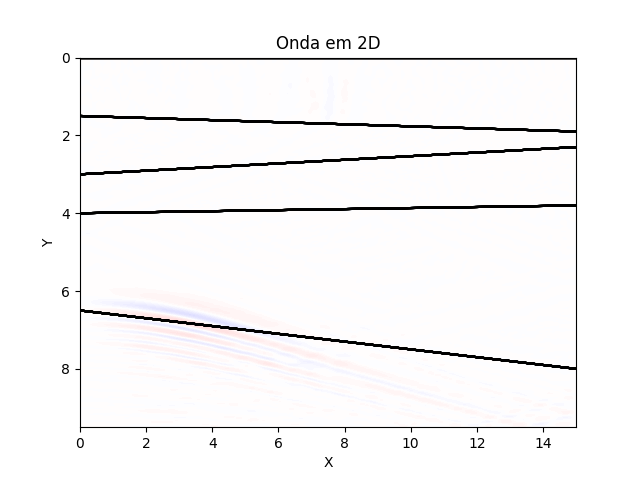
\includegraphics[width=65mm]{imagens/FDMimages/Teste023.png} &  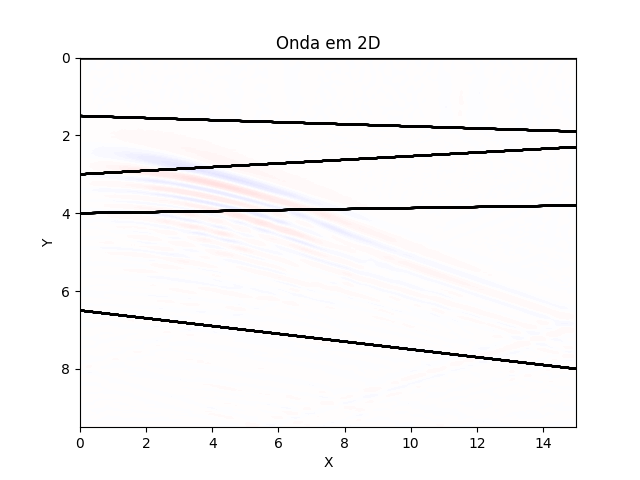
\includegraphics[width=65mm]{imagens/FDMimages/Teste030.png}\\
                    (e) 7 & (f) 8
                    \end{tabular}
                    \caption{\textit{Snapshots} da simulação numérica da propagação de uma onda}
                    \label{fig:snapsMDF}
                \end{figure}

                Na Figura \ref{fig:snapsMDF} podemos perceber que, como vimos no Capítulo \ref{cap:ond}, a cada vez que a onda encontra uma outra função de velocidades, ocorre uma refração e uma reflexão da onda. Por uma falha não ocorrem refrações e reflexões significantes nas camadas 3 e 4 pois, como se pode ver na Figura \ref{fig:velDist}, o gradiente de velocidades dessas camadas parece ser o mesmo.

	    \subsection{Domínio com Bordas ``Absorventes''}
	        
            Existem várias sugestões de implementações do método de diferenças finitas para a equação da onda com condições de contorno ``absorventes'' (ou ``abertas''). 
            
            Expandiremos o domínio de simulação de propagação das ondas, mas apresentaremos nas imagem apenas a parte que nos interessa. Dessa forma, durante a sua propagação, a onda não refletirá nas bordas da imagem como na seção anterior, mas dará a impressão de sair pelas bordas dela.
	        
            \subsubsection{Prática Numérica}
            
                Utilizando a mesma distribuição de velocidades visto na Figura \ref{fig:velDist}, obtemos a simulação demonstrada pelos \textit{snapshots} da Figura \ref{snapsMDFAbs}. Pode-se perceber que, ao contrário do caso das bordas refletoras, no caso atual, as frentes de onda passam além das extremidades da parte do meio que foi exibida. É como se o primeiro caso fosse um corpo caindo numa bacia de água, com o tempo, a superfície da possui um comportamento ondulatório complexo, com várias ondas se sobrepondo. Já o segundo o caso é como se o corpo caísse sobre a superfície do mar, onde não haveria bordas para as reflexões. Isso desconsiderando as reflexões que surgem com a passagem da frente de onda de uma camada para outra.
                
                \begin{figure}[H]
                    \begin{tabular}{cc}
                        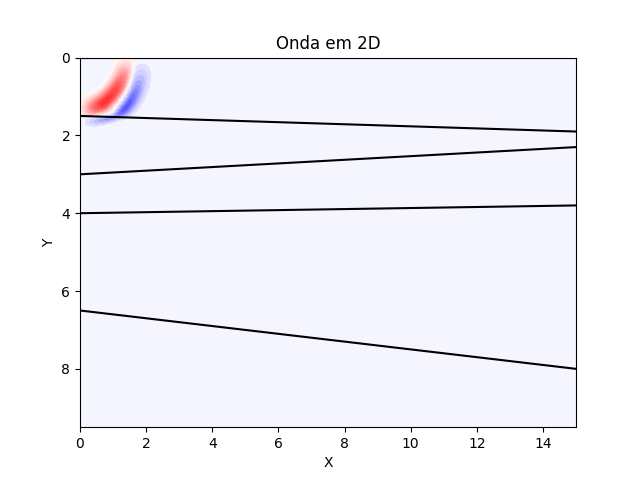
\includegraphics[width=65mm]{imagens/FDMimages/Teste00.png} & 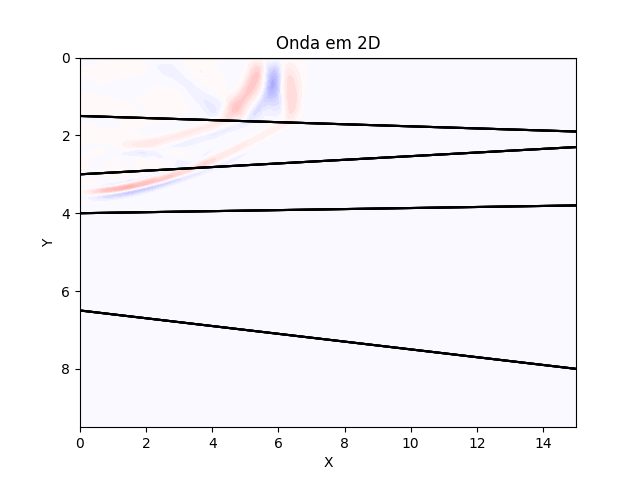
\includegraphics[width=65mm]{imagens/FDMimages/Teste03.png} \\
                        (a) 1 & (b) 2 \\
                        [6pt] 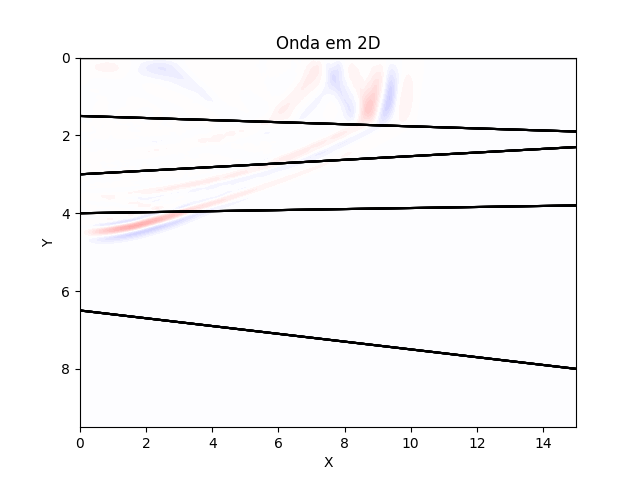
\includegraphics[width=65mm]{imagens/FDMimages/Teste05.png} & 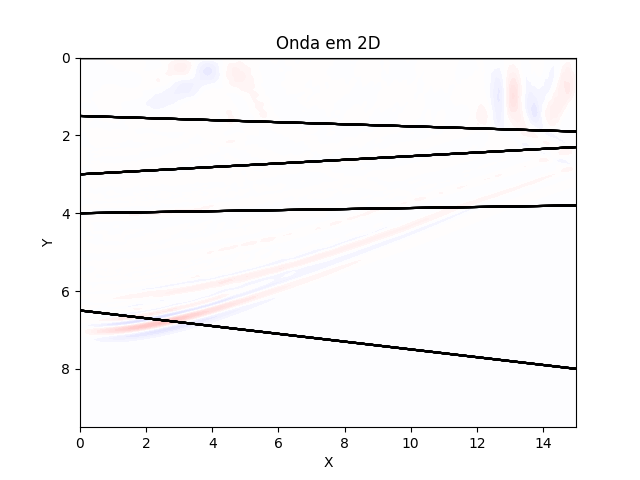
\includegraphics[width=65mm]{imagens/FDMimages/Teste010.png} \\
                        (c) 3 & (d) 4 \\
                        [6pt] 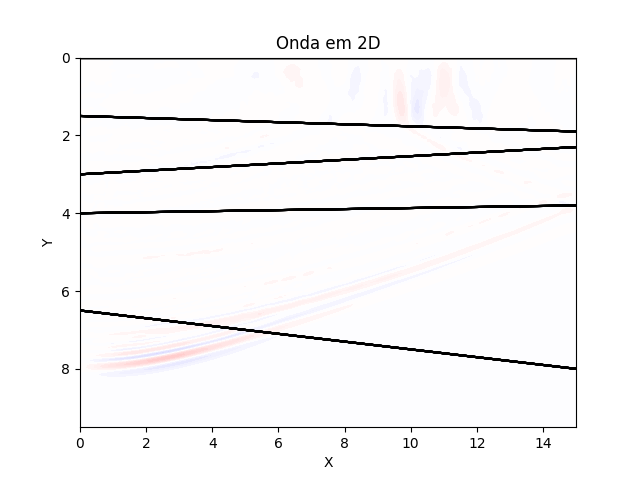
\includegraphics[width=65mm]{imagens/FDMimages/Teste012.png} & 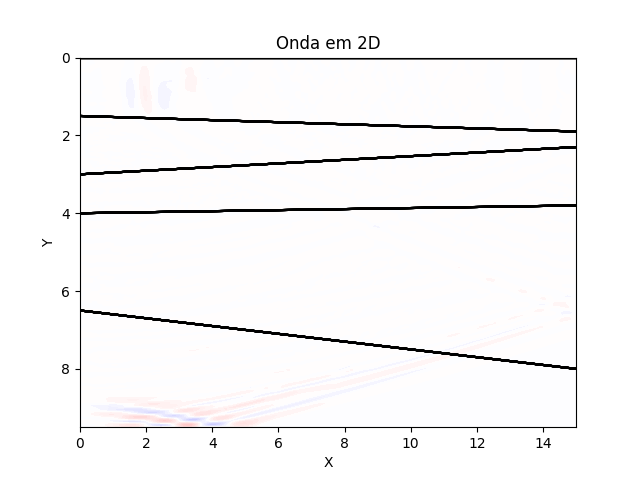
\includegraphics[width=65mm]{imagens/FDMimages/Teste017.png} \\ 
                        (e) 5 & (f) 6\\
                        [6pt] 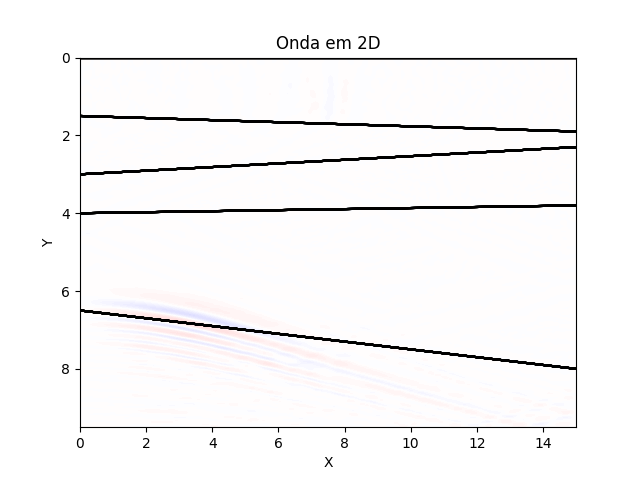
\includegraphics[width=65mm]{imagens/FDMimages/Teste023.png} & 
                        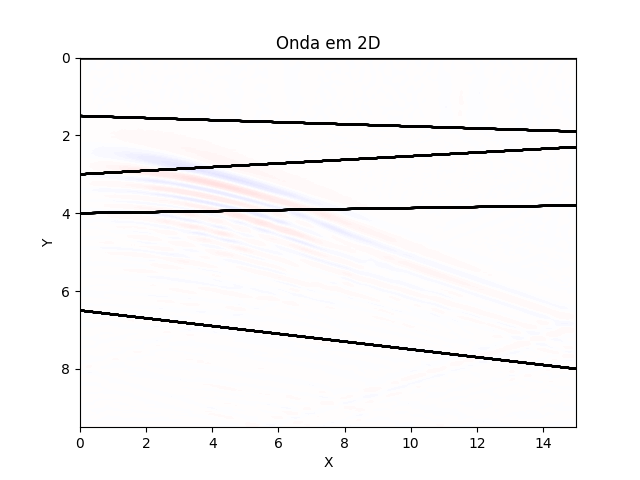
\includegraphics[width=65mm]{imagens/FDMimages/Teste030.png}\\
                        (e) 7 & (f) 8
                    \end{tabular}
                    \caption{\textit{Snapshots} da simulação numérica da propagação de uma onda.}
                    \label{snapsMDFAbs}
                \end{figure}

            
    \section{Resolução da Equação da Onda pelo Traçamento de Raios}
    
        \subsection{Implementação}
        
            Foi implementado um traçamento de raios simples, no qual há apenas uma reflexão nas interfaces que são definidas como refletoras. Neste traçamento, não são representadas as reflexões que ocorrem com as refrações.
            
            O raio é implementado como um \textit{array} de pontos que indicam sua posição $(x, y)$ no tempo $t$ e outro \textit{array} de componentes que constituem o vetor direção do raio ao longo do tempo. Já as interfaces são implementadas como retas em sua forma paramétrica: com um vetor diretor e um ponto. Além disso, a interface também possui um vetor normal.
        
            \subsubsection{O Traçamento}
            
                As posições e direções do raio ao longo do tempo são calculadas com o auxílio do método de Runge-Kutta de quarta ordem. Isso é feito porque o raio é definido matematicamente como um sistema de equações diferenciais para a posição e a direção ao longo do tempo.
                
                A interseção do raio com com a próxima interface se dá da seguinte forma: quando a função que implementa o método de Runge-Kutta percebe que o raio ultrapassou a interface, ela cria uma reta ligando os dois últimos pontos traçados para o raio e calcula a interseção dessa reta com a interface. O ponto de interseção calculado torna-se o último ponto do traçamento do raio para aquela camada.
            
            \subsubsection{Lei de Snell}
            
                Temos que a lei de Snell se dá por
                \begin{equation*}
                    \dfrac{\sin{\theta_2}}{\sin{\theta_1}} = \dfrac{v_2}{v_1} = \dfrac{n_1}{n_2}
                \end{equation*}
                na qual, $\theta_1$ e $\theta_2$ são os ângulos que, respectivamente, os raios incidente e refratado fazem com a normal, $v_1$ e $v_2$ são as velocidades dos meios acima e abaixo da reta preta (nas Figuras \ref{fig:reflect} e \ref{fig:refract}), respectivamente, assim como $n_1$ e $n_2$ são os coeficientes de refração de cada um, também respectivamente. A implementação da reflexão e da refração se baseiam nessa lei.
                
            \subsubsection{A Reflexão}
            
                Estando o raio sobre a interface que ele deve refletir, calculamos a projeção vetorial, $\vec{s}$, do último vetor direção, $\vec{p}$, do raio sobre a normal da interface. Após isso, somamos $\vec{p}$ com menos duas vezes $\vec{s}$ e obtemos o vetor direção refletido do raio. Também podemos visualizar isso pela seguinte imagem.
                
                \begin{figure}[H]
                    \centering 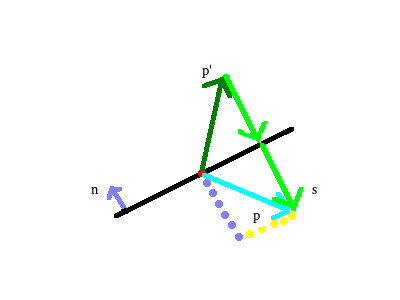
\includegraphics[scale=.8]{imagens/RTimages/reflect.png}
                    \caption{Esquema ilustrativo da reflexão do raio $\vec{p}$, em azul ciano, sobre uma interface, em preto. O vetor $\vec{s}$, em verde, é a projeção vetorial de $\vec{p}$ sobre o vetor normal $\vec{n}$ da interface, em lilás}
                    \label{fig:reflect}
                \end{figure}
            
            \subsubsection{A Refração}
            
                Estando o raio sobre uma interface não refletora, projetamos o vetor $\vec{p}$ sobre o vetor diretor $\vec{d}$ da interface. Dessa forma, sendo $\vec{p}$ um vetor unitário, obtemos o seno do ângulo da direção do raio naquele momento pela norma do vetor projetado. Com esse seno, aplicamos a lei de Snell e obtemos o seno do ângulo refratado. Então, pela seguinte igualdade trigonométrica
                \begin{equation*}
                    \cos{\theta} = \sqrt{1 - \sin^2{\theta}}
                \end{equation*}
                obtemos o cosseno do ângulo refratado. Assim, podemos multiplicar vetor $\vec{n}$ da interface pelo cosseno encontrado e somar esse vetor a $\vec{d}$ multiplicado pelo seno, obtendo então o novo vetor $\vec{p}$ do raio.
                
                \begin{figure}[H]
                    \centering
                    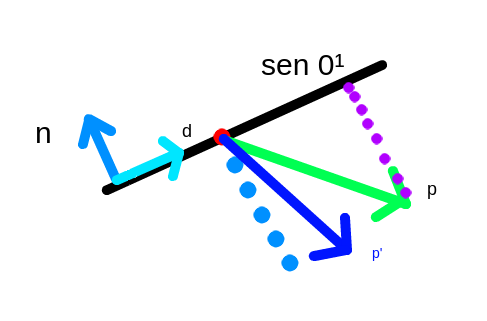
\includegraphics[scale=.6]{imagens/RTimages/refract.png}
                    
                    \hrulefill
                    \caption{Esquema ilustrativo da reflexão do raio $\vec{p}$, em verde, sobre uma interface, em preto. A norma da projeção de $\vec{p}$ sobre $\vec{d}$, em azul claro, é o seno do ângulo de $\vec{p}$ com a normal $\vec{n}$, em azul escuro. Após a aplicação da lei de Snell sobre esse seno, obtém-se o seno do ângulo refratado, que é usado para obter o cosseno do mesmo ângulo. Obtém-se $\vec{p'}$ multiplicando o cosseno e o seno encontrados por $\vec{n}$ e $\vec{d}$, respectivamente}
                    \hrulefill
                    \label{fig:refract}
                \end{figure}
            
        \subsection{Traçando Raios}
        
	        Utilizando a mesma distribuição de velocidades usada nos exemplos de implementação do método de diferenças finitas, podemos ver abaixo a simulação da propagação de ondas pelo mesmo meio das outras simulações, mas agora pelo método de traçamento de raios. Os ângulos mínimo e máximo de emisão dos raios foram, respectivamente, 10º e 18º. A cada encontro do raio com uma interface podemos ver uma refração (calculada usando a função velocidade das duas camadas naquele ponto), exceto na última interface.
	        
            \begin{figure}[H]
            	\centering
            	\label{RTsim01}
            	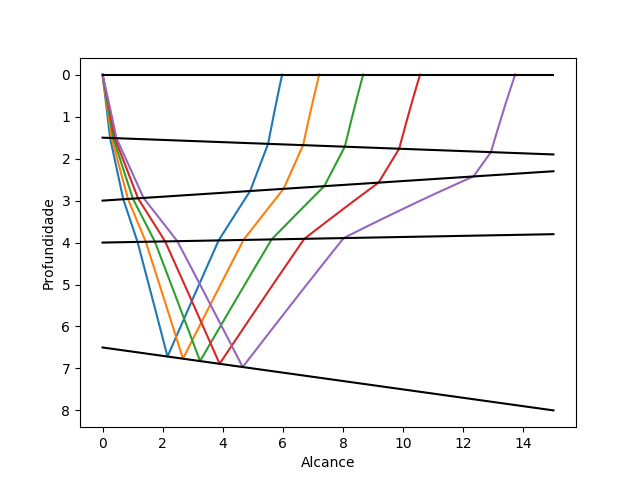
\includegraphics[scale=.6]{imagens/RTimages/sim01.png}
            	\caption{Simulação da propagação de ondas pelo método do traçamento de raios}
            \end{figure}
            
            \begin{figure}[H]
               	\centering
               	\label{RTsim02}
               	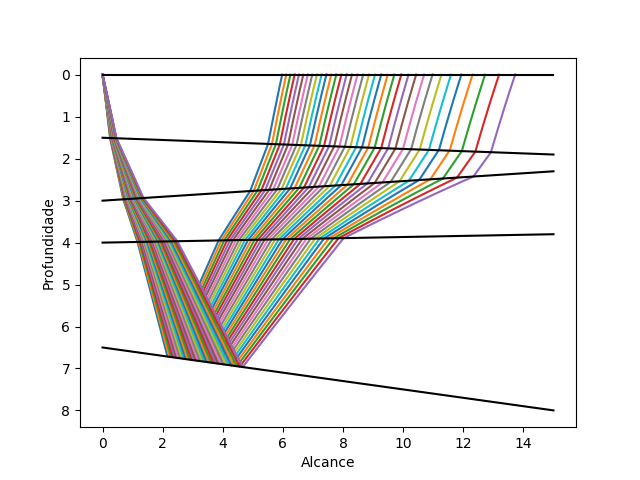
\includegraphics[scale=.6]{imagens/RTimages/sim02.png}
               	\caption{A mesma simulação que a Figura \ref{RTsim01} exibe, mas agora com 35 raios}
            \end{figure}
            
            \newpage
            Podemos ver pelas simulações seguintes que é também possível decidir sobre qual interface os raios devem refletir. Isso é útil para se observar como se dá a reflexão sobre cada interface
            \begin{figure}[H]
               	\centering
               	\label{RTsim03}
               	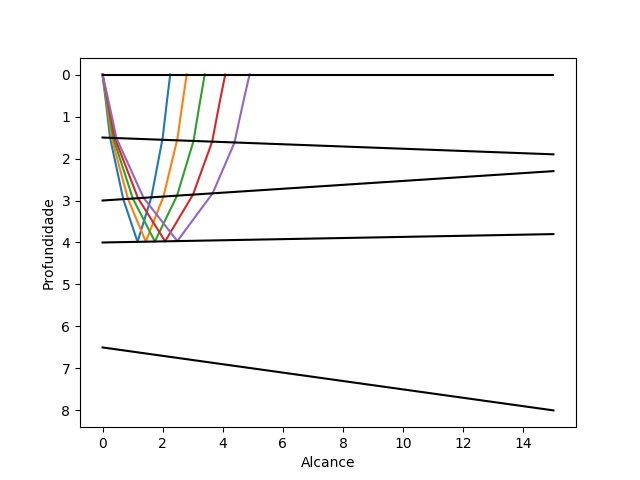
\includegraphics[scale=.6]{imagens/RTimages/sim03.png}
               	\caption{Traçamento de raios com reflexão na terceira interface}
            \end{figure}
            
			\begin{figure}[H]
               	\centering
               	\label{RTsim04}
               	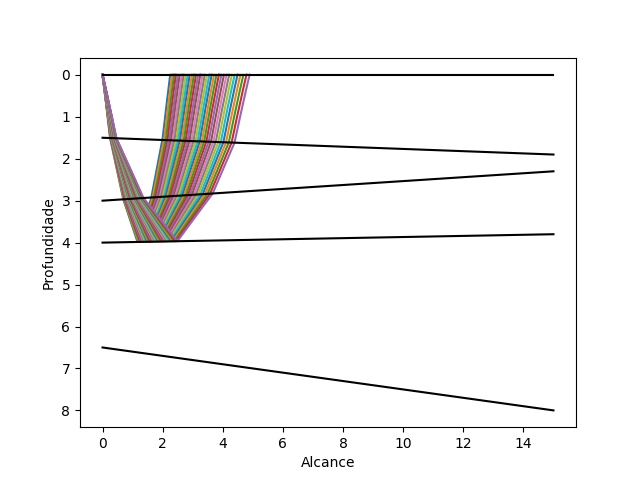
\includegraphics[scale=.6]{imagens/RTimages/sim04.png}
               	\caption{O mesmo traçamento da Figura \ref{RTsim03}, mas agora com mais raios}
			\end{figure}
            
    \section{Comparação Entre os Métodos}
    
        Tanto o método de diferenças finitas quanto o traçamento de raios possuem suas vantagens e desvantagens. Durante a execução deste trabalho pude notar as seguintes características sobre cada uma dessas abordagens para a simulação de propagação de ondas.
        
        \subsection{Método das Diferenças Finitas}
        
            Possui uma forma fácil de se implementar, necessitando-se apenas conhecer os conceitos de derivadas parciais e diferenças finitas, que são relativamente fáceis. Para para a resolução numérica de um problema de equações diferenciais parciais, como a da onda, bastam poucas linhas de código. O uso da biblioteca \textit{Numpy} possibilita isso, além de acelerar os tratamentos numéricos no processo.
            
            Além disso, o a visualização da transformação dos dados, através do tempo, possibilitada método e pelas bibliotecas gráficas permite entender, intuitivamente, que a equação da onda é um modelo que imita bem o fenômeno físico. Essa visualização, em pequena escala, poderia ser utilizada na ministração de aulas de Cálculo Numérico, Métodos Numéricos Computacionais e/ou Física.
            
            Contudo, o processo de simulação por esse método tem um preço alto para grandes domínios (bem como da visualização gráfica de seus dados, que pode custar mais ainda). É comum que, para evitar instabilidades numéricas tenha-se que aumentar o número de pontos no \textit{array}, para que os passos dados pelo método não sejam muito grandes. Isso afeta a quantidade de memória e de processamento (e, consequentemente, de tempo e de recursos financeiros) necessária para a execução da simulação a tal ponto que, para uma simulação na área de Sismologia, por exemplo, que tem um grande volume de dados, a utilização do método se torna inviável.
            
        \subsection{Traçamento de Raios}
        
            A teoria do traçamento de raios é, matematicamente, complicada e nada intuitiva nos primeiros contatos. A implementação em código do traçamento também segue isso, sendo repleta de condicionais e cuidados que devem ser levados em conta. É necessária uma boa compreensão da teoria matemática antes da implementação do método, bem como a paciência com os erros que aparecerão e tempo para a implementação dos detalhes do traçamento.
            
            Contudo, imitar uma parte infinitesimal da frente de onda ao invés de simulá-la completamente é muito mais eficiente e menos custoso. Ou seja, o uso do traçamento de raios gasta menos memória (basta armazenar, além do meio e suas informações, as informações dos raios) e processamento (não é necessária computação sobre um grande \textit{array} tridimensional, mas apenas os \textit{arrays} de posição e direção dos raios) que o método de diferenças finitas para fazer, fundamentalmente, a mesma coisa. É por isso que o traçamento é uma das técnicas mais utilizadas nos ramos como a já citada Sismologia.
            
            Por fim, até mesmo a exibição gráfica dos dados do traçamento, pelo menos em pequena escala como feito nesse projeto, é mais rápida do que no caso da exibição dos dados conseguidos pelo método anterior, visto que exibe-se ``linhas'' e não malhas inteiras.